% This file is generated by the MATLAB m-file laprint.m. It can be included
% into LaTeX documents using the packages graphicx, color and psfrag.
% It is accompanied by a postscript file. A sample LaTeX file is:
%    \documentclass{article}\usepackage{graphicx,color,psfrag}
%    \begin{document}% This file is generated by the MATLAB m-file laprint.m. It can be included
% into LaTeX documents using the packages graphicx, color and psfrag.
% It is accompanied by a postscript file. A sample LaTeX file is:
%    \documentclass{article}\usepackage{graphicx,color,psfrag}
%    \begin{document}% This file is generated by the MATLAB m-file laprint.m. It can be included
% into LaTeX documents using the packages graphicx, color and psfrag.
% It is accompanied by a postscript file. A sample LaTeX file is:
%    \documentclass{article}\usepackage{graphicx,color,psfrag}
%    \begin{document}% This file is generated by the MATLAB m-file laprint.m. It can be included
% into LaTeX documents using the packages graphicx, color and psfrag.
% It is accompanied by a postscript file. A sample LaTeX file is:
%    \documentclass{article}\usepackage{graphicx,color,psfrag}
%    \begin{document}\input{batt_load_exp}\end{document}
% See http://www.mathworks.de/matlabcentral/fileexchange/loadFile.do?objectId=4638
% for recent versions of laprint.m.
%
% created by:           LaPrint version 3.16 (13.9.2004)
% created on:           18-Feb-2014 21:34:20
% eps bounding box:     15 cm x 8.1771 cm
% comment:              
%
\begin{psfrags}%
\psfragscanon%
%
% text strings:
\psfrag{s05}[t][t]{\color[rgb]{0,0,0}\setlength{\tabcolsep}{0pt}\begin{tabular}{c}Time (seconds)\end{tabular}}%
\psfrag{s06}[b][b]{\color[rgb]{0,0,0}\setlength{\tabcolsep}{0pt}\begin{tabular}{c}$\mathrm{V_{cell}}$\end{tabular}}%
\psfrag{s07}[b][b]{\color[rgb]{0,0,0}\setlength{\tabcolsep}{0pt}\begin{tabular}{c}Time Series Plot:$\mathrm{V_{cell}}$\end{tabular}}%
\psfrag{s08}[t][t]{\color[rgb]{0,0,0}\setlength{\tabcolsep}{0pt}\begin{tabular}{c}Time (seconds)\end{tabular}}%
\psfrag{s09}[b][b]{\color[rgb]{0,0,0}\setlength{\tabcolsep}{0pt}\begin{tabular}{c}$\mathrm{i_{cell}}$\end{tabular}}%
\psfrag{s10}[b][b]{\color[rgb]{0,0,0}\setlength{\tabcolsep}{0pt}\begin{tabular}{c}Time Series Plot:$\mathrm{i_{cell}}$\end{tabular}}%
\psfrag{s11}[t][t]{\color[rgb]{0,0,0}\setlength{\tabcolsep}{0pt}\begin{tabular}{c}Time (seconds)\end{tabular}}%
\psfrag{s12}[b][b]{\color[rgb]{0,0,0}\setlength{\tabcolsep}{0pt}\begin{tabular}{c}$R_L$\end{tabular}}%
%
% xticklabels:
\psfrag{x01}[t][t]{0}%
\psfrag{x02}[t][t]{5000}%
\psfrag{x03}[t][t]{10000}%
\psfrag{x04}[t][t]{15000}%
\psfrag{x05}[t][t]{0}%
\psfrag{x06}[t][t]{5000}%
\psfrag{x07}[t][t]{10000}%
\psfrag{x08}[t][t]{15000}%
\psfrag{x09}[t][t]{0}%
\psfrag{x10}[t][t]{5000}%
\psfrag{x11}[t][t]{10000}%
\psfrag{x12}[t][t]{15000}%
%
% yticklabels:
\psfrag{v01}[r][r]{-6}%
\psfrag{v02}[r][r]{-4}%
\psfrag{v03}[r][r]{-2}%
\psfrag{v04}[r][r]{0}%
\psfrag{v05}[r][r]{2}%
\psfrag{v06}[r][r]{4}%
\psfrag{v07}[r][r]{6}%
\psfrag{v08}[r][r]{-1}%
\psfrag{v09}[r][r]{-0.5}%
\psfrag{v10}[r][r]{0}%
\psfrag{v11}[r][r]{0.5}%
\psfrag{v12}[r][r]{1}%
\psfrag{v13}[r][r]{2}%
\psfrag{v14}[r][r]{2.5}%
\psfrag{v15}[r][r]{3}%
\psfrag{v16}[r][r]{3.5}%
\psfrag{v17}[r][r]{4}%
\psfrag{v18}[r][r]{4.5}%
%
% Figure:
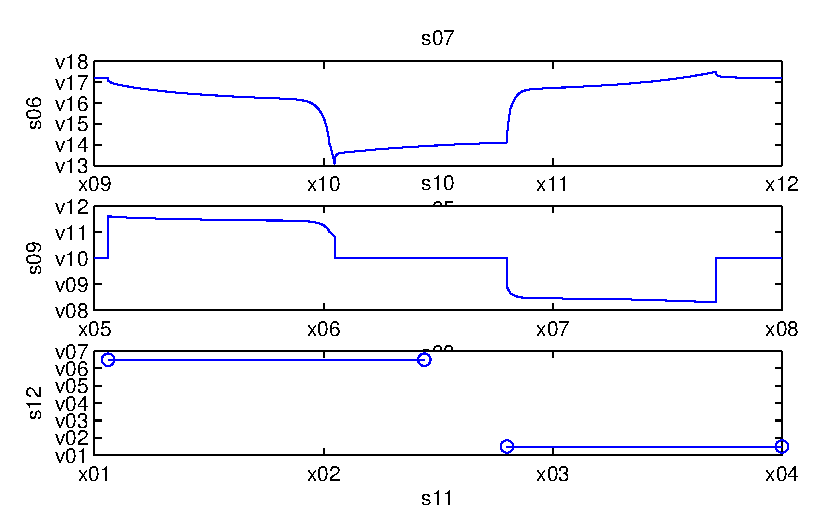
\includegraphics[width=12cm]{batt_load_exp.eps}%
\end{psfrags}%
%
% End batt_load_exp.tex
\end{document}
% See http://www.mathworks.de/matlabcentral/fileexchange/loadFile.do?objectId=4638
% for recent versions of laprint.m.
%
% created by:           LaPrint version 3.16 (13.9.2004)
% created on:           18-Feb-2014 21:34:20
% eps bounding box:     15 cm x 8.1771 cm
% comment:              
%
\begin{psfrags}%
\psfragscanon%
%
% text strings:
\psfrag{s05}[t][t]{\color[rgb]{0,0,0}\setlength{\tabcolsep}{0pt}\begin{tabular}{c}Time (seconds)\end{tabular}}%
\psfrag{s06}[b][b]{\color[rgb]{0,0,0}\setlength{\tabcolsep}{0pt}\begin{tabular}{c}$\mathrm{V_{cell}}$\end{tabular}}%
\psfrag{s07}[b][b]{\color[rgb]{0,0,0}\setlength{\tabcolsep}{0pt}\begin{tabular}{c}Time Series Plot:$\mathrm{V_{cell}}$\end{tabular}}%
\psfrag{s08}[t][t]{\color[rgb]{0,0,0}\setlength{\tabcolsep}{0pt}\begin{tabular}{c}Time (seconds)\end{tabular}}%
\psfrag{s09}[b][b]{\color[rgb]{0,0,0}\setlength{\tabcolsep}{0pt}\begin{tabular}{c}$\mathrm{i_{cell}}$\end{tabular}}%
\psfrag{s10}[b][b]{\color[rgb]{0,0,0}\setlength{\tabcolsep}{0pt}\begin{tabular}{c}Time Series Plot:$\mathrm{i_{cell}}$\end{tabular}}%
\psfrag{s11}[t][t]{\color[rgb]{0,0,0}\setlength{\tabcolsep}{0pt}\begin{tabular}{c}Time (seconds)\end{tabular}}%
\psfrag{s12}[b][b]{\color[rgb]{0,0,0}\setlength{\tabcolsep}{0pt}\begin{tabular}{c}$R_L$\end{tabular}}%
%
% xticklabels:
\psfrag{x01}[t][t]{0}%
\psfrag{x02}[t][t]{5000}%
\psfrag{x03}[t][t]{10000}%
\psfrag{x04}[t][t]{15000}%
\psfrag{x05}[t][t]{0}%
\psfrag{x06}[t][t]{5000}%
\psfrag{x07}[t][t]{10000}%
\psfrag{x08}[t][t]{15000}%
\psfrag{x09}[t][t]{0}%
\psfrag{x10}[t][t]{5000}%
\psfrag{x11}[t][t]{10000}%
\psfrag{x12}[t][t]{15000}%
%
% yticklabels:
\psfrag{v01}[r][r]{-6}%
\psfrag{v02}[r][r]{-4}%
\psfrag{v03}[r][r]{-2}%
\psfrag{v04}[r][r]{0}%
\psfrag{v05}[r][r]{2}%
\psfrag{v06}[r][r]{4}%
\psfrag{v07}[r][r]{6}%
\psfrag{v08}[r][r]{-1}%
\psfrag{v09}[r][r]{-0.5}%
\psfrag{v10}[r][r]{0}%
\psfrag{v11}[r][r]{0.5}%
\psfrag{v12}[r][r]{1}%
\psfrag{v13}[r][r]{2}%
\psfrag{v14}[r][r]{2.5}%
\psfrag{v15}[r][r]{3}%
\psfrag{v16}[r][r]{3.5}%
\psfrag{v17}[r][r]{4}%
\psfrag{v18}[r][r]{4.5}%
%
% Figure:
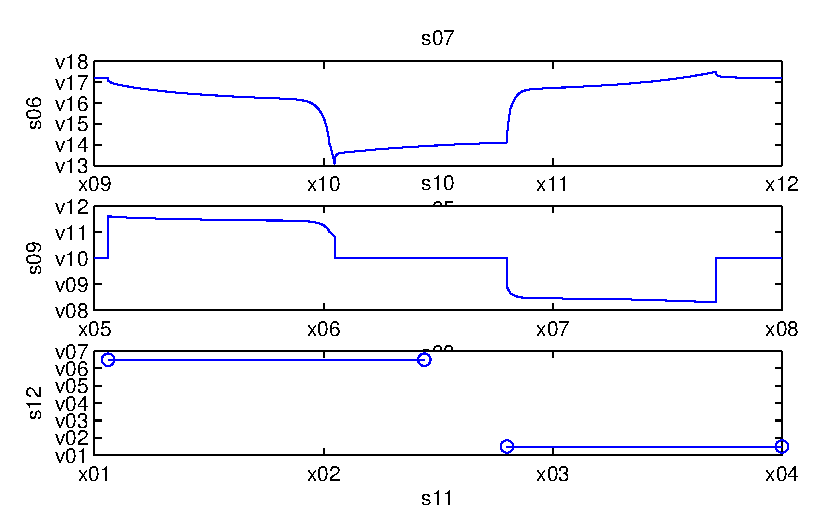
\includegraphics[width=12cm]{batt_load_exp.eps}%
\end{psfrags}%
%
% End batt_load_exp.tex
\end{document}
% See http://www.mathworks.de/matlabcentral/fileexchange/loadFile.do?objectId=4638
% for recent versions of laprint.m.
%
% created by:           LaPrint version 3.16 (13.9.2004)
% created on:           18-Feb-2014 21:34:20
% eps bounding box:     15 cm x 8.1771 cm
% comment:              
%
\begin{psfrags}%
\psfragscanon%
%
% text strings:
\psfrag{s05}[t][t]{\color[rgb]{0,0,0}\setlength{\tabcolsep}{0pt}\begin{tabular}{c}Time (seconds)\end{tabular}}%
\psfrag{s06}[b][b]{\color[rgb]{0,0,0}\setlength{\tabcolsep}{0pt}\begin{tabular}{c}$\mathrm{V_{cell}}$\end{tabular}}%
\psfrag{s07}[b][b]{\color[rgb]{0,0,0}\setlength{\tabcolsep}{0pt}\begin{tabular}{c}Time Series Plot:$\mathrm{V_{cell}}$\end{tabular}}%
\psfrag{s08}[t][t]{\color[rgb]{0,0,0}\setlength{\tabcolsep}{0pt}\begin{tabular}{c}Time (seconds)\end{tabular}}%
\psfrag{s09}[b][b]{\color[rgb]{0,0,0}\setlength{\tabcolsep}{0pt}\begin{tabular}{c}$\mathrm{i_{cell}}$\end{tabular}}%
\psfrag{s10}[b][b]{\color[rgb]{0,0,0}\setlength{\tabcolsep}{0pt}\begin{tabular}{c}Time Series Plot:$\mathrm{i_{cell}}$\end{tabular}}%
\psfrag{s11}[t][t]{\color[rgb]{0,0,0}\setlength{\tabcolsep}{0pt}\begin{tabular}{c}Time (seconds)\end{tabular}}%
\psfrag{s12}[b][b]{\color[rgb]{0,0,0}\setlength{\tabcolsep}{0pt}\begin{tabular}{c}$R_L$\end{tabular}}%
%
% xticklabels:
\psfrag{x01}[t][t]{0}%
\psfrag{x02}[t][t]{5000}%
\psfrag{x03}[t][t]{10000}%
\psfrag{x04}[t][t]{15000}%
\psfrag{x05}[t][t]{0}%
\psfrag{x06}[t][t]{5000}%
\psfrag{x07}[t][t]{10000}%
\psfrag{x08}[t][t]{15000}%
\psfrag{x09}[t][t]{0}%
\psfrag{x10}[t][t]{5000}%
\psfrag{x11}[t][t]{10000}%
\psfrag{x12}[t][t]{15000}%
%
% yticklabels:
\psfrag{v01}[r][r]{-6}%
\psfrag{v02}[r][r]{-4}%
\psfrag{v03}[r][r]{-2}%
\psfrag{v04}[r][r]{0}%
\psfrag{v05}[r][r]{2}%
\psfrag{v06}[r][r]{4}%
\psfrag{v07}[r][r]{6}%
\psfrag{v08}[r][r]{-1}%
\psfrag{v09}[r][r]{-0.5}%
\psfrag{v10}[r][r]{0}%
\psfrag{v11}[r][r]{0.5}%
\psfrag{v12}[r][r]{1}%
\psfrag{v13}[r][r]{2}%
\psfrag{v14}[r][r]{2.5}%
\psfrag{v15}[r][r]{3}%
\psfrag{v16}[r][r]{3.5}%
\psfrag{v17}[r][r]{4}%
\psfrag{v18}[r][r]{4.5}%
%
% Figure:
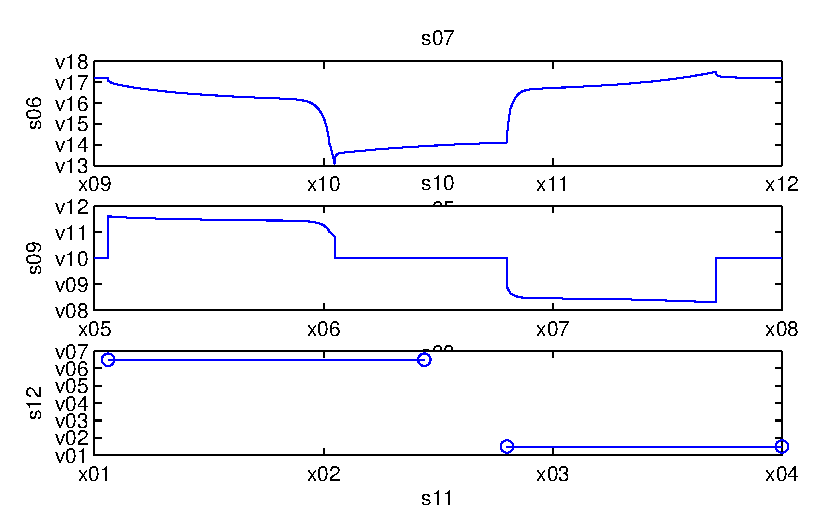
\includegraphics[width=12cm]{batt_load_exp.eps}%
\end{psfrags}%
%
% End batt_load_exp.tex
\end{document}
% See http://www.mathworks.de/matlabcentral/fileexchange/loadFile.do?objectId=4638
% for recent versions of laprint.m.
%
% created by:           LaPrint version 3.16 (13.9.2004)
% created on:           18-Feb-2014 21:34:20
% eps bounding box:     15 cm x 8.1771 cm
% comment:              
%
\begin{psfrags}%
\psfragscanon%
%
% text strings:
\psfrag{s05}[t][t]{\color[rgb]{0,0,0}\setlength{\tabcolsep}{0pt}\begin{tabular}{c}Time (seconds)\end{tabular}}%
\psfrag{s06}[b][b]{\color[rgb]{0,0,0}\setlength{\tabcolsep}{0pt}\begin{tabular}{c}V_{cell}\end{tabular}}%
\psfrag{s07}[b][b]{\color[rgb]{0,0,0}\setlength{\tabcolsep}{0pt}\begin{tabular}{c}Time Series Plot:V_{cell}\end{tabular}}%
\psfrag{s08}[t][t]{\color[rgb]{0,0,0}\setlength{\tabcolsep}{0pt}\begin{tabular}{c}Time (seconds)\end{tabular}}%
\psfrag{s09}[b][b]{\color[rgb]{0,0,0}\setlength{\tabcolsep}{0pt}\begin{tabular}{c}i_{cell}\end{tabular}}%
\psfrag{s10}[b][b]{\color[rgb]{0,0,0}\setlength{\tabcolsep}{0pt}\begin{tabular}{c}Time Series Plot:i_{cell}\end{tabular}}%
\psfrag{s11}[t][t]{\color[rgb]{0,0,0}\setlength{\tabcolsep}{0pt}\begin{tabular}{c}Time (seconds)\end{tabular}}%
\psfrag{s12}[b][b]{\color[rgb]{0,0,0}\setlength{\tabcolsep}{0pt}\begin{tabular}{c}R_L\end{tabular}}%
%
% xticklabels:
\psfrag{x01}[t][t]{0}%
\psfrag{x02}[t][t]{5000}%
\psfrag{x03}[t][t]{10000}%
\psfrag{x04}[t][t]{15000}%
\psfrag{x05}[t][t]{0}%
\psfrag{x06}[t][t]{5000}%
\psfrag{x07}[t][t]{10000}%
\psfrag{x08}[t][t]{15000}%
\psfrag{x09}[t][t]{0}%
\psfrag{x10}[t][t]{5000}%
\psfrag{x11}[t][t]{10000}%
\psfrag{x12}[t][t]{15000}%
%
% yticklabels:
\psfrag{v01}[r][r]{-6}%
\psfrag{v02}[r][r]{-4}%
\psfrag{v03}[r][r]{-2}%
\psfrag{v04}[r][r]{0}%
\psfrag{v05}[r][r]{2}%
\psfrag{v06}[r][r]{4}%
\psfrag{v07}[r][r]{6}%
\psfrag{v08}[r][r]{-1}%
\psfrag{v09}[r][r]{-0.5}%
\psfrag{v10}[r][r]{0}%
\psfrag{v11}[r][r]{0.5}%
\psfrag{v12}[r][r]{1}%
\psfrag{v13}[r][r]{2}%
\psfrag{v14}[r][r]{2.5}%
\psfrag{v15}[r][r]{3}%
\psfrag{v16}[r][r]{3.5}%
\psfrag{v17}[r][r]{4}%
\psfrag{v18}[r][r]{4.5}%
%
% Figure:
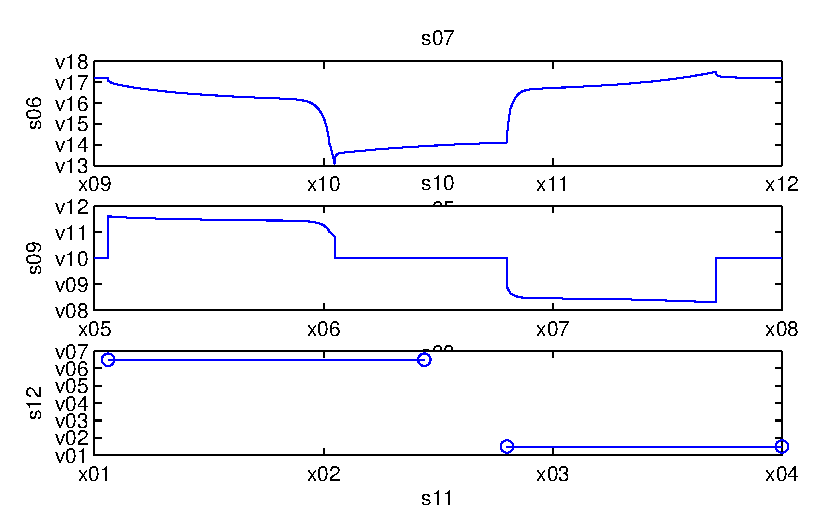
\includegraphics[width=12cm]{batt_load_exp.eps}%
\end{psfrags}%
%
% End batt_load_exp.tex
